\documentclass[12pt]{beamer}
\usepackage[utf8]{inputenc}
\usepackage[T1]{fontenc}
\usepackage{lmodern}
\usepackage{ngerman}
\usepackage{amsmath}
\usepackage{amsfonts}
\usepackage{amssymb}
\usepackage{graphicx}
\usepackage{pgfplots}
\usepackage{geometry}
\usepackage{fancyhdr}
\usepackage{lastpage}
\usepackage{float}
\usepackage{tikz}
\usepackage[european,smartlabels,siunitx]{circuitikz}
\usetikzlibrary{calc,positioning}

\pgfdeclareimage[width = 1.5cm]{meinlogo}{Logo.png}

\usetheme{CambridgeUS}
\usecolortheme{seagull}

\begin{document}
	\author[Gruppe D]{\textbf{Marcel Sandermann}, Micha Beyer, Patrick Schlüter}
	\title{Kantenerkennung}
	\subtitle{Projekt 1}
	\logo{\pgfuseimage{meinlogo}}
	\institute[HS OWL]{Hochschule Ostwestfalen Lippe}
	\date{31.10.2018}
	%\subject{was das}
	%\setbeamercovered{transparent}
	\setbeamertemplate{navigation symbols}{}
	
	
\begin{frame}
	\titlepage
\end{frame}

\begin{frame}
	\frametitle{Inhalt}
	\tableofcontents	
\end{frame}

\section{Einleitung}
\subsection{Problemstellung}
\begin{frame}
	\frametitle{Problemstellung}
	\begin{itemize}
		\item Kanten einer gegebenen Zellstruktur sollen erkannt werden
		\item Übergangsbereich ist undefiniert		
	\end{itemize}
	\begin{columns}[c]
		\column{.5\textwidth}
		\begin{figure}
		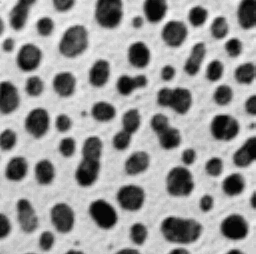
\includegraphics[width=0.5\linewidth]{Anfang.png}
		\caption{Ausgangssituation}	
		\end{figure}
		\column{.5\textwidth}
		\begin{figure}
			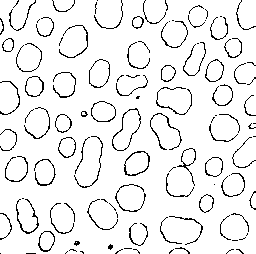
\includegraphics[width=0.5\linewidth]{Ergebnis.png}
			\caption{Ergebnis}
		\end{figure}		 	
	\end{columns}	
\end{frame}

\section{Lösungsweg}
\subsection{Punktoperation \& Schwellwerterkennung}

\begin{frame}
\frametitle{Punktoperation}
\begin{itemize}
	\item Festlegung der Schwellwerte
	\item Jeder Pixel wird einzelnd betrachtet
	\item Kantenerkennung via Schwellwerterkennung
\end{itemize}
\begin{block}{Schwellwerterkennung}	
	\begin{equation*}
		f_{treshold}=
		\begin{cases}
			a_0   			& \text{für } a < q_1,\\
			a_1        		& \text{für } q_1 \leq a \leq q_2, \\
			a_0        		& \text{für } q_2 < a,
		\end{cases}
	\end{equation*}
\end{block}
\end{frame}
\subsection{Javaprogramm}
\begin{frame}
	\begin{figure}[H]
		\centering
		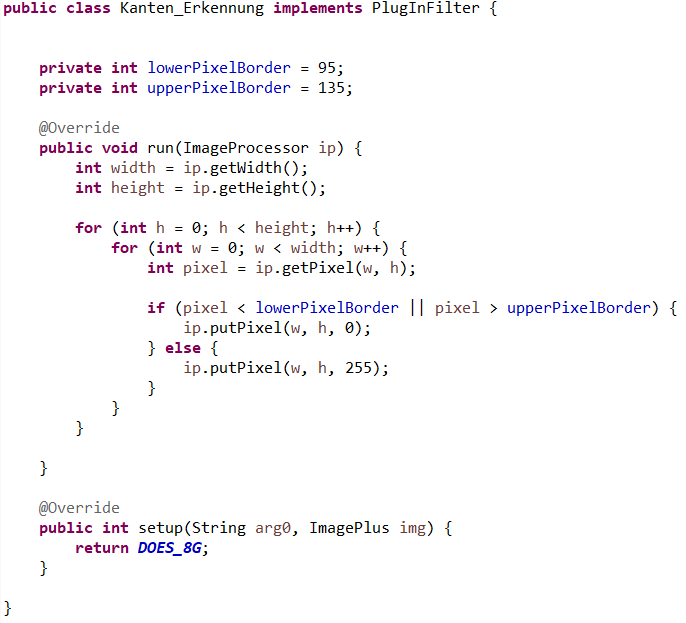
\includegraphics[width=.6\linewidth]{Code.png}
		\caption{Java-Code zur Schwellwertbearbeitung}
	\end{figure}
\end{frame}

\section{Fazit}

\begin{frame}
	\frametitle{Fazit}
	\begin{itemize}
		\item Keine wirkliche Kantenerkennung 
		\begin{itemize}
			\item Kante besteht aus mehreren Pixeln
		\end{itemize}
		\item \textbf{Punktoperation für diese Anwendung nicht sinnvoll}		
	\end{itemize}
\end{frame}

\section*{}

\begin{frame}
	\frametitle{Referenzen}
	\Large{Vielen Dank für eure Aufmerksamkeit}	
	\newline
	\begin{block}{Quellen}
		\small{	
		\begin{thebibliography}{99} % Beamer does not support BibTeX so references must be inserted manually as below
			\bibitem[Burger, Burge, 2015]{p1} Wilhelm Burger, Mark James Burge (2015)
			\newblock Digitale Bildverarbeitung: Eine algorithmische Einführung mit Java
			%\newblock \emph{Journal Name} 12(3), 45 -- 678.
		\end{thebibliography}
		}
	\end{block}
\end{frame}

\end{document}